\documentclass[aspectratio=169]{beamer}
\usepackage{UAH-theme}
\usepackage{minted}
\usepackage{xcolor}
% Use a placeholder if you don't have the actual logo
% Create a simple UAH logo placeholder
\usepackage{tikz}
\usepackage{array}
\usepackage{multirow}
\usepackage{array}
\usepackage{colortbl}
\usepackage{booktabs}

\usetikzlibrary{arrows.meta, positioning}
\definecolor{stackaddr}{RGB}{173,216,230}
\definecolor{stackval}{RGB}{255,228,181}
\definecolor{stackdesc}{RGB}{144,238,144}
\definecolor{addr}{RGB}{173,216,230}
\definecolor{val}{RGB}{255,228,181}
\definecolor{desc}{RGB}{144,238,144}

\newcommand{\UAHLogoPlaceholder}{%
\begin{tikzpicture}[scale=0.15]
\draw[fill=UAHred,draw=none] (0,0) circle (5);
\draw[white,line width=0.5mm] (0,0) circle (4);
\draw[white,line width=0.5mm] (-2,2) -- (2,2);
\draw[white,line width=0.5mm] (-2,-2) -- (2,-2);
\draw[white,line width=0.5mm] (0,4) -- (0,-4);
\end{tikzpicture}%
}

\definecolor{frame1}{RGB}{255, 230, 230}
\definecolor{frame2}{RGB}{230, 255, 230}
\definecolor{frame3}{RGB}{230, 230, 255}
\definecolor{frame4}{RGB}{255, 255, 230}

\usemintedstyle{default}
\setminted{
fontsize=\footnotesize,
frame=single,
linenos=true,
breaklines=true,
autogobble=true
}

\title{ARM Assembly: Stack Frames and Frame Pointers Demo}
\subtitle{CPE 221}
\author{Rahul Bhadani}
\institute{The University of Alabama in Huntsville}
\date{March 16, 2025}

\begin{document}

\begin{frame}

    \titlepage

\end{frame}

\begin{frame}{}
    \tableofcontents
\end{frame}

\begin{frame}{Introduction}
    \begin{itemize}
    \item ARM Assembly program with 4 nested function calls
    \item Assume base address of SP as $0x2000$
    \item Each function has its own stack frame
    \item Visualizing stack and frame pointers during execution
    \end{itemize}
    
\end{frame}

    \begin{frame}{Stack Organization in ARM}
    \begin{itemize}
    \item Stack grows downward in memory
    \item SP (Stack Pointer) - Points to the current top of stack
    \item FP (R11) - Frame Pointer, maintains reference to current frame
    \item Each function:
        \begin{itemize}
        \item Saves previous FP and LR (Link Register)
        \item Sets up new frame with local variables
        \item Restores previous frame on exit
        \end{itemize}
    \end{itemize}
    \end{frame}

        

\section{C++ Implementation}

\begin{frame}[fragile]{C++ Implementation - Main Function}
    \begin{minted}[fontsize=\tiny]{cpp}
#include <iostream>

// Function prototypes
int firstFunction(int a);
int secondFunction(int b);
int thirdFunction(int c);
int fourthFunction(int d);

int main() {
    int inputValue = 8;
    std::cout << "Starting with value: " << inputValue << std::endl;
    std::cout << "------------------------" << std::endl;
    
    int finalResult = firstFunction(inputValue);
    
    std::cout << "------------------------" << std::endl;
    std::cout << "Final result: " << finalResult << std::endl;
    
    return 0;
}
    \end{minted}
\end{frame}

\begin{frame}[fragile]{C++ Implementation - First Function}
    \begin{minted}[fontsize=\tiny]{cpp}
// First function (outermost)
int firstFunction(int a) {
    // Four local variables
    int localVar1 = a + 15;
    int localVar2 = a * 3;
    int localVar3 = a << 3;  // Bit shift left by 3 (multiply by 8)
    int localVar4 = 100;
    
    // Call the second function
    int nestedResult = secondFunction(localVar2 + a);
    
    // Final calculation
    int result = localVar1 * localVar4 + nestedResult - localVar3;
    
    std::cout << "First function: " << a << " -> " << result << std::endl;
    return result;
}

\end{minted}
\end{frame}

\begin{frame}[fragile]{C++ Implementation - Second Function}
    \begin{minted}[fontsize=\tiny]{cpp}

// Second function
int secondFunction(int b) {
    // Four local variables
    int localVar1 = b << 1;  // Bit shifting (multiplication by 2)
    int localVar2 = b + b;
    int localVar3 = b * b;
    int localVar4 = 12;
    
    // Call the third function
    int nestedResult = thirdFunction(localVar1 - localVar4);
    
    // Some bitwise operations for variety
    int result = nestedResult & localVar3 | localVar2;
    
    std::cout << "Second function: " << b << " -> " << result << std::endl;
    return result;
}
    \end{minted}
\end{frame}

\begin{frame}[fragile]{C++ Implementation - Third Function}
    \begin{minted}[fontsize=\tiny]{cpp}
// Third function
int thirdFunction(int c) {
    // Four local variables
    int localVar1 = c * 3;
    int localVar2 = c - 5;
    int localVar3 = c + 7;
    int localVar4 = 7;
    
    // Call the fourth function
    int nestedResult = fourthFunction(localVar1 + localVar2);
    
    // More math operations
    int result = nestedResult + (localVar3 * localVar4);
    
    std::cout << "Third function: " << c << " -> " << result << std::endl;
    return result;
}

\end{minted}
\end{frame}

\begin{frame}[fragile]{C++ Implementation - Fourth Function}
    \begin{minted}[fontsize=\tiny]{cpp}

// Fourth function (innermost)
int fourthFunction(int d) {
    // Four local variables
    int localVar1 = d * 2;
    int localVar2 = d + 10;
    int localVar3 = d * d;
    int localVar4 = 5;
    
    // Some interesting math: Compute a polynomial expression
    int result = localVar1 * localVar3 + localVar2 * localVar4;
    
    std::cout << "Fourth function: " << d << " -> " << result << std::endl;
    return result;
}
    \end{minted}
\end{frame}

\section{ARM Assembly Implementation}

\begin{frame}[fragile]{ARM Assembly - Program Entry}
    \begin{minted}[fontsize=\tiny]{bash}
@ ARMv7 Assembly implementation of the nested function calls program
@ Using SP for stack pointer and FP (R11) for frame pointer

.text
.global _START

_START:
    LDR SP, =0x2000        // Initialize stack pointer
    MOV R0, #8             // inputValue = 8
    SUB SP, SP, #8         // Allocate space for inputValue + finalResult
    STR R0, [SP, #4]       // Store inputValue at 0x1FFC
    BL FIRSTFUNCTION       // Call FIRSTFUNCTION
    STR R0, [SP]           // Store finalResult at 0x1FF8
DONE:  B DONE              // Infinite loop
    \end{minted}
\end{frame}

\begin{frame}[fragile]{ARM Assembly - First Function}
    \begin{minted}[fontsize=\tiny]{bash}
    FIRSTFUNCTION:
        PUSH {FP, LR}          // Save FP and LR
        MOV FP, SP             // FP = current SP
        SUB SP, SP, #24        // Allocate 24 bytes for locals
    
        // CORRECTED: Load inputValue from [FP, #12] instead of [FP, #8]
        LDR R0, [FP, #12]      // Load inputValue from 0x1FFC
        ADD R1, R0, #15        // localVar1 = a + 15
        STR R1, [FP, #-24]     // Store localVar1 at [FP-24]
    
    
        // localVar2 = a * 3
        MOV R1, #3             // Load 3 into R1
        MUL R1, R0, R1         // localVar2 = a * 3
        STR R1, [FP, #-20]     // Store localVar2 at [FP-20]
    
        // localVar3 = a << 3
        LSL R1, R0, #3         // localVar3 = a << 3
        STR R1, [FP, #-16]     // Store localVar3 at [FP-16]
    
        // localVar4 = 100
        MOV R1, #100           // localVar4 = 100
        STR R1, [FP, #-12]     // Store localVar4 at [FP-12]
    
        // Call SECONDFUNCTION(localVar2 + a)
        LDR R1, [FP, #-20]     // Load localVar2
        ADD R0, R1, R0         // R0 = localVar2 + a
        BL SECONDFUNCTION      // Call SECONDFUNCTION
        STR R0, [FP, #-8]      // Store nestedResult at [FP-8]
\end{minted}
\end{frame}

\begin{frame}[fragile]{ARM Assembly - First Function (continued)}
    \begin{minted}[fontsize=\tiny]{bash}

    // Calculate final result
        LDR R1, [FP, #-24]     // Load localVar1
        LDR R2, [FP, #-12]     // Load localVar4
        MUL R3, R1, R2         // R3 = localVar1 * localVar4
        LDR R1, [FP, #-8]      // Load nestedResult
        ADD R3, R3, R1         // R3 += nestedResult
        LDR R1, [FP, #-16]     // Load localVar3
        SUB R0, R3, R1         // R0 = R3 - localVar3
        STR R0, [FP, #-4]      // Store result at [FP-4]
        LDR R0, [FP, #-4]      // Load result into R0
    
        MOV SP, FP             // Epilogue: Restore SP
        POP {FP, PC}           // Restore FP and return
    \end{minted}
\end{frame}

\begin{frame}[fragile]{ARM Assembly - Second Function}
    \begin{minted}[fontsize=\tiny]{bash}
    SECONDFUNCTION:
        PUSH {FP, LR}          // Prologue: Save FP and LR
        MOV FP, SP             // Set FP to current SP
        SUB SP, SP, #24        // Allocate 24 bytes for locals
    
        // localVar1 = b << 1
        LSL R1, R0, #1         // localVar1 = b << 1
        STR R1, [FP, #-24]     // Store localVar1 at [FP-24]
    
        // localVar2 = b + b
        ADD R1, R0, R0         // localVar2 = b + b
        STR R1, [FP, #-20]     // Store localVar2 at [FP-20]
    
        // localVar3 = b * b
        MUL R1, R0, R0         // localVar3 = b * b
        STR R1, [FP, #-16]     // Store localVar3 at [FP-16]
    
        // localVar4 = 12
        MOV R1, #12            // localVar4 = 12
        STR R1, [FP, #-12]     // Store localVar4 at [FP-12]
\end{minted}
\end{frame}

\begin{frame}[fragile]{ARM Assembly - Second Function (continued)}
    \begin{minted}[fontsize=\tiny]{bash}

    // Call THIRDFUNCTION(localVar1 - localVar4)
        LDR R1, [FP, #-24]     // Load localVar1
        LDR R2, [FP, #-12]     // Load localVar4
        SUB R0, R1, R2         // R0 = localVar1 - localVar4
        BL THIRDFUNCTION       // Call THIRDFUNCTION
        STR R0, [FP, #-8]      // Store nestedResult at [FP-8]
    
        // Calculate result
        LDR R1, [FP, #-8]      // Load nestedResult
        LDR R2, [FP, #-16]     // Load localVar3
        AND R3, R1, R2         // R3 = nestedResult & localVar3
        LDR R1, [FP, #-20]     // Load localVar2
        ORR R0, R3, R1         // R0 = R3 | localVar2
        STR R0, [FP, #-4]      // Store result at [FP-4]
        LDR R0, [FP, #-4]      // Load result into R0
    
        MOV SP, FP             // Epilogue: Restore SP
        POP {FP, PC}           // Restore FP and return
    \end{minted}
\end{frame}

\begin{frame}[fragile]{ARM Assembly - Third Function}
    \begin{minted}[fontsize=\tiny]{bash}
    THIRDFUNCTION:
        PUSH {FP, LR}          // Prologue: Save FP and LR
        MOV FP, SP             // Set FP to current SP
        SUB SP, SP, #24        // Allocate 24 bytes for locals
    
        // localVar1 = c * 3
        MOV R1, #3             // Load 3 into R1
        MUL R1, R0, R1         // localVar1 = c * 3
        STR R1, [FP, #-24]     // Store localVar1 at [FP-24]
    
        // localVar2 = c - 5
        SUB R1, R0, #5         // localVar2 = c - 5
        STR R1, [FP, #-20]     // Store localVar2 at [FP-20]
    
        // localVar3 = c + 7
        ADD R1, R0, #7         // localVar3 = c + 7
        STR R1, [FP, #-16]     // Store localVar3 at [FP-16]
    
        // localVar4 = 7
        MOV R1, #7             // localVar4 = 7
        STR R1, [FP, #-12]     // Store localVar4 at [FP-12]
    
\end{minted}
\end{frame}

\begin{frame}[fragile]{ARM Assembly - Third Function (continued)}
    \begin{minted}[fontsize=\tiny]{bash}

    // Call FOURTHFUNCTION(localVar1 + localVar2)
        LDR R1, [FP, #-24]     // Load localVar1
        LDR R2, [FP, #-20]     // Load localVar2
        ADD R0, R1, R2         // R0 = localVar1 + localVar2
        BL FOURTHFUNCTION      // Call FOURTHFUNCTION
        STR R0, [FP, #-8]      // Store nestedResult at [FP-8]
    
        // Calculate result
        LDR R1, [FP, #-16]     // Load localVar3
        LDR R2, [FP, #-12]     // Load localVar4
        MUL R3, R1, R2         // R3 = localVar3 * localVar4
        LDR R1, [FP, #-8]      // Load nestedResult
        ADD R0, R1, R3         // R0 = nestedResult + R3
        STR R0, [FP, #-4]      // Store result at [FP-4]
        LDR R0, [FP, #-4]      // Load result into R0
    
        MOV SP, FP             // Epilogue: Restore SP
        POP {FP, PC}           // Restore FP and return
    \end{minted}
\end{frame}

\begin{frame}[fragile]{ARM Assembly - Fourth Function}
    \begin{minted}[fontsize=\tiny]{bash}
    FOURTHFUNCTION:
        PUSH {FP, LR}          // Prologue: Save FP and LR
        MOV FP, SP             // Set FP to current SP
        SUB SP, SP, #24        // Allocate 24 bytes for locals
    
        // localVar1 = d * 2
        LSL R1, R0, #1         // localVar1 = d * 2
        STR R1, [FP, #-24]     // Store localVar1 at [FP-24]
    
        // localVar2 = d + 10
        ADD R1, R0, #10        // localVar2 = d + 10
        STR R1, [FP, #-20]     // Store localVar2 at [FP-20]
    
        // localVar3 = d * d
        MUL R1, R0, R0         // localVar3 = d * d
        STR R1, [FP, #-16]     // Store localVar3 at [FP-16]
    
        // localVar4 = 5
        MOV R1, #5             // localVar4 = 5
        STR R1, [FP, #-12]     // Store localVar4 at [FP-12]

\end{minted}
\end{frame}

\begin{frame}[fragile]{ARM Assembly - Fourth Function (continued)}
    \begin{minted}[fontsize=\tiny]{bash}

    // Calculate result
        LDR R1, [FP, #-24]     // Load localVar1
        LDR R2, [FP, #-16]     // Load localVar3
        MUL R3, R1, R2         // R3 = localVar1 * localVar3
        LDR R1, [FP, #-20]     // Load localVar2
        LDR R2, [FP, #-12]     // Load localVar4
        MUL R2, R1, R2         // R2 = localVar2 * localVar4
        ADD R0, R3, R2         // R0 = R3 + R2
        STR R0, [FP, #-8]      // Store result at [FP-8]
        LDR R0, [FP, #-8]      // Load result into R0
    
        MOV SP, FP             // Epilogue: Restore SP
        POP {FP, PC}           // Restore FP and return
    \end{minted}
\end{frame}


\section{Stack Frame Analysis During Program Execution}


\begin{frame}{Program Initialization}
    \begin{table}[h]
        \centering
        \begin{tabular}{|>{\columncolor{stackaddr}}l|>{\columncolor{stackval}}l|>{\columncolor{stackdesc}}l|}
        \hline
        \textbf{Address} & \textbf{Content} & \textbf{Description} \\
        \hline
        0x2000 & SP\_init & Initial stack pointer \\
        \hline
        0x1FFC & 8 & inputValue (R0) \\
        \hline
        0x1FF8 & (empty) & Reserved for finalResult \\
        \hline
        \end{tabular}
    \end{table}

    
    
    \begin{itemize}
    \item SP initialized to 0x2000
    \item SP adjusted to 0x1FF8 (SP - 8 bytes)
    \item R0 = 8 (inputValue) stored at [SP, \#-4]
    \item Now ready to call firstFunction with R0 = 8
    \end{itemize}
\end{frame}

\begin{frame}{FIRSTFUNCTION Stack Frame}
    \begin{table}[h]
    \centering
    \begin{tabular}{|>{\columncolor{stackaddr}}l|>{\columncolor{stackval}}l|>{\columncolor{stackdesc}}l|}
    \hline
    \textbf{Address} & \textbf{Content} & \textbf{Description} \\
    \hline
    0x1FF4 & LR & Return address \\
    \hline
    0x1FF0 & Old FP & Previous frame pointer \\
    \hline
    0x1FEC & result & Final calculation \\
    \hline
    0x1FE8 & nestedResult & From SECONDFUNCTION \\
    \hline
    0x1FE4 & 100 & localVar4 \\
    \hline
    0x1FE0 & 64 & localVar3 a$<<$3 \\
    \hline
    0x1FDC & 24 & a*3 localVar2 \\    \hline
    0x1FD8 & 23 & a+15 localVar1 \\
    \hline
    \end{tabular}
    \end{table}
    

\end{frame}
    
    % ==================== SECOND FUNCTION ====================
\begin{frame}{SECONDFUNCTION Stack Frame}
    \begin{table}[h]
    \centering
    \begin{tabular}{|>{\columncolor{addr}}l|>{\columncolor{val}}l|>{\columncolor{desc}}l|}
    \hline
    \textbf{Address} & \textbf{Content} & \textbf{Description} \\
    \hline
    0x1FD4 & LR & Return to FIRSTFUNCTION \\  \hline
    0x1FD0 & Old FP & Previous frame pointer \\  \hline
    0x1FCC &  & Final result \\  \hline
    0x1FC8 &  & nestedResult \\  \hline
    0x1FC4 &  & localVar4\\  \hline
    0x1FC0 &  &  localVar3 (b * b)  \\  \hline
    0x1FBC &  & localVar2 (b + b) \\  \hline
    0x1FB8 &  & localVar1 (b $<< $1)  \\  \hline
    \end{tabular}
    \end{table}
    

    \begin{itemize}
    \item Bitwise AND/OR operations
    \item Receives parameter from FIRSTFUNCTION
    \end{itemize}
    \end{frame}
    
    % ==================== THIRD FUNCTION ====================
    \begin{frame}{THIRDFUNCTION Stack Frame}
    \begin{table}[h]
    \centering
    \begin{tabular}{|>{\columncolor{addr}}l|>{\columncolor{val}}l|>{\columncolor{desc}}l|}
    \hline
    \textbf{Address} & \textbf{Content} & \textbf{Description} \\
    \hline
    0x1FB4 & LR & Return to SECONDFUNCTION \\  \hline
    0x1FB0 & Old FP & Previous frame pointer \\  \hline
    0x1FAC &  &  Final result \\  \hline
    0x1FA8 &  &  nestedResult \\  \hline
    0x1FA4 &  & localVar4\\  \hline
    0x1FA0 &  &  localVar3 (c + 7)  \\  \hline
    0x1F9C &  & localVar2 (c - 5) \\  \hline
    0x1F98 &  & localVar1 (c * 3) \\  \hline
    \end{tabular}
    \end{table}
    

    \begin{itemize}
    \item Calls FOURTHFUNCTION
    \end{itemize}
    \end{frame}
    
    % ==================== FOURTH FUNCTION ====================
    \begin{frame}{FOURTHFUNCTION Stack Frame}
    \begin{table}[h]
    \centering
    \begin{tabular}{|>{\columncolor{addr}}l|>{\columncolor{val}}l|>{\columncolor{desc}}l|}
    \hline
    \textbf{Address} & \textbf{Content} & \textbf{Description} \\
    \hline
    0x1F94 & LR & Return to THIRDFUNCTION \\
    0x1F90 & Old FP & Previous frame pointer \\
    0x1F8C &  & Final result\\
    0x1F88 &  &  localVar4 \\
    0x1F84 & & localVar3 (d * d) \\
    0x1F80 &  & localVar2 (d + 10)\\
    0x1F7C &  &  localVar1 (d * 2) \\
    \hline
    \end{tabular}
    \end{table}
    
    \begin{itemize}
    \item Innermost function
    \end{itemize}
    \end{frame}
    
    % ==================== FINAL _START FRAME ====================
    \begin{frame}{Final \_START Stack State}
    \begin{table}[h]
    \centering
    \begin{tabular}{|>{\columncolor{addr}}l|>{\columncolor{val}}l|>{\columncolor{desc}}l|}
    \hline
    \textbf{Address} & \textbf{Content} & \textbf{Description} \\
    \hline
    0x2000 & (SP init) & Original stack top \\
    0x1FFC & 8 & Preserved inputValue \\
    0x1FF8 & 2300 & Final result \\
    0x1FF4 & ... & Cleaned stack space \\
    \hline
    \end{tabular}
    \end{table}
    

    \begin{itemize}
    \item SP returns to 0x1FF8 after functions unwind
    \item 8-byte allocation remains with final result
    \item All temporary stack frames cleaned
    \end{itemize}
    \end{frame}
    
    % ==================== STACK GROWTH DIAGRAM ====================
    \begin{frame}{Complete Stack Growth Diagram}
        \tiny
    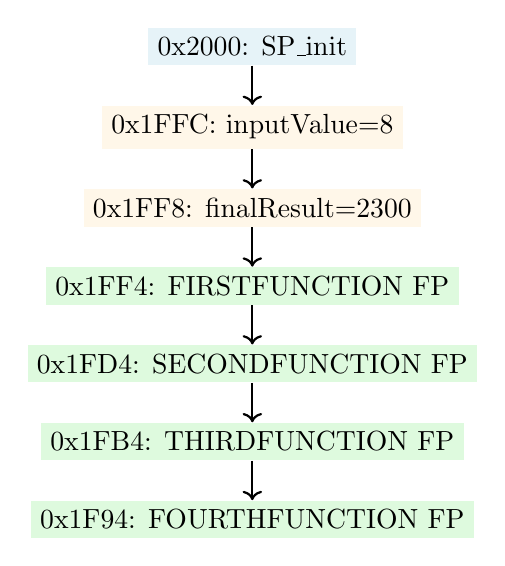
\begin{tikzpicture}[node distance=0.5cm]
    \node (start) [rectangle,fill=addr!30] {0x2000: SP\_init};
    \node (input) [rectangle,fill=val!30, below=of start] {0x1FFC: inputValue=8};
    \node (result) [rectangle,fill=val!30, below=of input] {0x1FF8: finalResult=2300};
    \node (f1) [rectangle,fill=desc!30, below=of result] {0x1FF4: FIRSTFUNCTION FP};
    \node (f2) [rectangle,fill=desc!30, below=of f1] {0x1FD4: SECONDFUNCTION FP};
    \node (f3) [rectangle,fill=desc!30, below=of f2] {0x1FB4: THIRDFUNCTION FP};
    \node (f4) [rectangle,fill=desc!30, below=of f3] {0x1F94: FOURTHFUNCTION FP};
    
    \draw[->,thick] (start) -- (input);
    \draw[->,thick] (input) -- (result);
    \draw[->,thick] (result) -- (f1);
    \draw[->,thick] (f1) -- (f2);
    \draw[->,thick] (f2) -- (f3);
    \draw[->,thick] (f3) -- (f4);
    \end{tikzpicture}
    
    \begin{itemize}
    \item Total stack depth: 0x2000 - 0x1F94 = 108 bytes
    \item Each function frame uses 28 bytes (7×4)
    \item Stack unwinds completely except for final result
    \end{itemize}
    \end{frame}
    

    
\end{document}